\documentclass[tikz,border=4pt]{standalone}
\usetikzlibrary{arrows.meta,positioning,calc}
\begin{document}
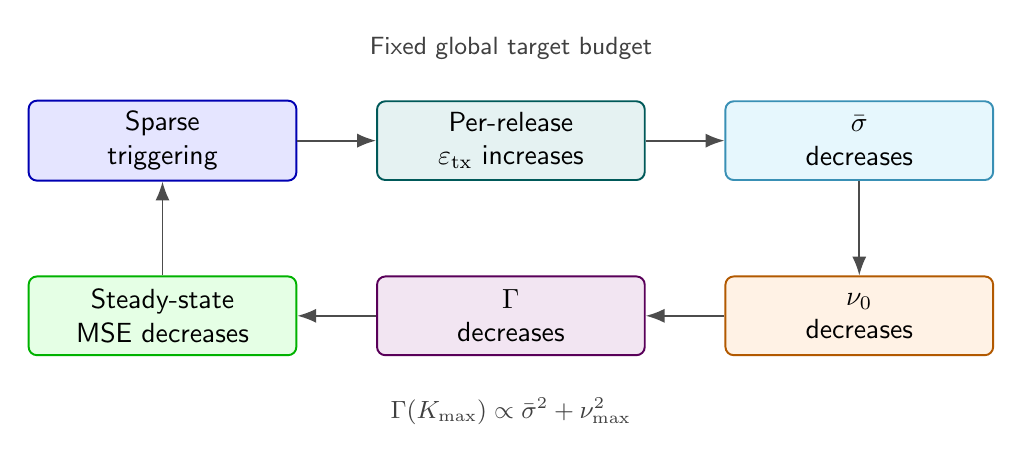
\begin{tikzpicture}[
  font=\sffamily,
  box/.style={draw=#1!70!black, fill=#1!10, rounded corners=3pt, line width=0.7pt,
    align=center, minimum width=34mm, minimum height=10mm, inner sep=4pt},
  arrow/.style={-{Latex[length=2.4mm]}, line width=0.65pt, draw=black!70},
  note/.style={font=\sffamily\small, align=center, text=black!75}
]
  \node[box=blue] (sparse) {Sparse\\triggering};
  \node[box=teal, right=10mm of sparse] (eps) {Per-release\\$\varepsilon_{\mathrm{tx}}$ increases};
  \node[box=cyan, right=10mm of eps] (noise) {$\bar{\sigma}$\\decreases};
  \node[box=orange, below=12mm of noise] (resid) {$\nu_0$\\decreases};
  \node[box=violet, left=10mm of resid] (gamma) {$\Gamma$\\decreases};
  \node[box=green, left=10mm of gamma] (mse) {Steady-state\\MSE decreases};

  \draw[arrow] (sparse) -- (eps);
  \draw[arrow] (eps) -- (noise);
  \draw[arrow] (noise) -- (resid);
  \draw[arrow] (resid) -- (gamma);
  \draw[arrow] (gamma) -- (mse);
  \draw[arrow, rounded corners=8pt] (mse.north) |- ($(sparse.south)+(0,-5mm)$) -| (sparse.south);

  \node[note, above=4mm of eps] {Fixed global target budget};
  \node[note, below=4mm of gamma] {$\Gamma(K_{\max})\propto\bar{\sigma}^{2}+\nu_{\max}^{2}$};
\end{tikzpicture}
\end{document}
